\documentclass[fleqn, a4paper, 12pt, oneside]{amsart}
\usepackage{exsheets, tasks}
\usepackage{amsmath, amssymb, amsthm} %standard AMS packages
\usepackage{marginnote} %marginnotes
\usepackage{gensymb} %miscellaneous symbols
\usepackage{commath} %differential symbols
\usepackage{xcolor} %colours
\usepackage{cancel} %cancelling terms
\usepackage{siunitx} %formatting units
\usepackage{tikz, pgfplots} %diagrams
\usetikzlibrary{calc, hobby, patterns, intersections}
\usepackage{graphicx} %inserting graphics
\usepackage{hyperref} %hyperlinks
\usepackage{datetime} %date and time
\usepackage{ulem} %underline for \emph{}
\usepackage{xfrac} %inline fractions
\usepackage{enumerate} %numbered lists
\usepackage{float} %inserting floats
\usepackage{circuitikz} %circuit diagrams

\newcommand\numberthis{\addtocounter{equation}{1}\tag{\theequation}} %adds numbers to specific equations in non-numbered list of equations

\newcommand{\AxisRotator}[1][rotate=0]{
	\tikz [x=0.25cm,y=0.60cm,line width=.2ex,-stealth,#1] \draw (0,0) arc (-150:150:1 and 1);%
} %rotation symbols on axes

\theoremstyle{definition}
\newtheorem{example}{Example}
\newtheorem{definition}{Definition}

\theoremstyle{theorem}
\newtheorem{theorem}{Theorem}

\newcommand{\curl}{\mathrm{curl\,}}

\makeatletter
\@addtoreset{section}{part} %resets section numbers in new part
\makeatother

\renewcommand{\thesubsection}{(\arabic{subsection})}
\renewcommand{\thesection}{(\arabic{section})}

%section headings on left
\makeatletter
\def\specialsection{\@startsection{section}{1}%
	\z@{\linespacing\@plus\linespacing}{.5\linespacing}%
	%  {\normalfont\centering}}% DELETED
	{\normalfont}}% NEW
\def\section{\@startsection{section}{1}%
	\z@{.7\linespacing\@plus\linespacing}{.5\linespacing}%
	%  {\normalfont\scshape\centering}}% DELETED
	{\normalfont\scshape}}% NEW
\makeatother

%forces newline after subsection
\makeatletter
\def\subsection{\@startsection{subsection}{3}%
	\z@{.5\linespacing\@plus.7\linespacing}{.1\linespacing}%
	{\normalfont\itshape}}
\makeatother

\settasks{counter-format = tsk[1].}

\SetupExSheets{solution/print = true}

%opening
\title{Physics 2 : Assignment 1}
\author
{
	Aakash Jog\\
	ID : 989323563
}
\date{\formatdate{18}{3}{2015}}

\begin{document}
	
\maketitle
%\setlength{\mathindent}{0pt}

\begin{question}
	\begin{tasks}
		\task
			Twelve equal charges, $q$, are situated at the comers of a regular 12- sided polygon (for instance, one on each numeral of a clock face). What is the net force on a test charge $Q$ at the centre?
		\task
			Suppose one of the 12 $q$s is removed (the one at ``6 o'clock"). What is the force on $Q$? Explain your reasoning carefully.
		\task
			Now 13 equal charges, $q$, are placed at the comers of a regular 13-sided polygon. What is the force on a test charge $Q$ at the centre?
		\task
			If one of the 13 $q$s is removed, what is the force on $Q$? Explain your reasoning.
	\end{tasks}
\end{question}

\begin{solution}
	\begin{tasks}
		\task
			\begin{figure}[H]
				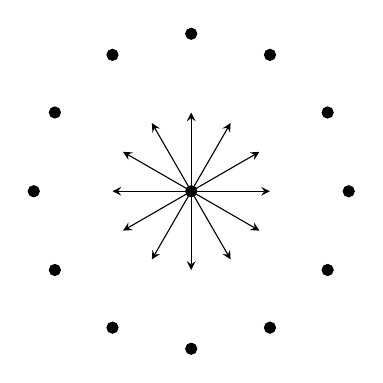
\begin{tikzpicture}
					\def\R{2};
					
					\foreach \i in {1,...,12}
					{
						\filldraw ({\i*360/12}:\R) circle [radius = 2pt];
						\draw [-stealth] (0,0) -- ($ (0,0) ! -1cm ! ({\i*360/12}:\R)$);
					}
					
					\filldraw (0,0) circle [radius = 2pt];
				\end{tikzpicture}
			\end{figure}
			
			The vector sum of the forces shown above is zero. Therefore, the net force acting on $Q$ is zero.
		\task
			\begin{figure}[H]
				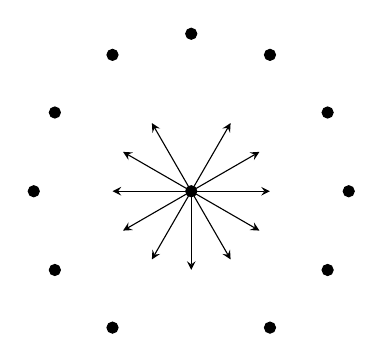
\begin{tikzpicture}
					\def\R{2};
					
					\foreach \i in {1,...,8,10,11,12}
					{
						\filldraw ({\i*360/12}:\R) circle [radius = 2pt];
						\draw [-stealth] (0,0) -- ($ (0,0) ! -1cm ! ({\i*360/12}:\R)$);
					}
					
					\filldraw (0,0) circle [radius = 2pt];
				\end{tikzpicture}
			\end{figure}
			
			All of the forces, except for force due to the charge at 12 o'clock, are cancelled out. Hence the net force is
			\begin{align*}
				\overrightarrow{F} &= k \dfrac{Q q}{R^2}
			\end{align*}
			in the 6 o'clock direction.
			
		\task
			\begin{figure}[H]
				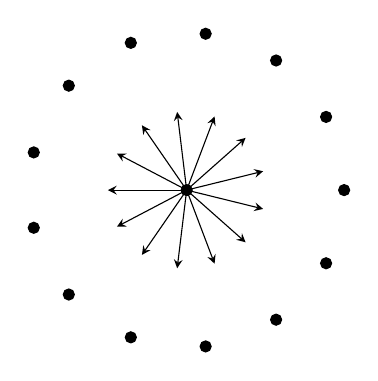
\begin{tikzpicture}
					\def\R{2};
					
					\foreach \i in {1,...,13}
					{
						\filldraw ({\i*360/13}:\R) circle [radius = 2pt];
						\draw [-stealth] (0,0) -- ($ (0,0) ! -1cm ! ({\i*360/13}:\R)$);
					}
					
					\filldraw (0,0) circle [radius = 2pt];
				\end{tikzpicture}
			\end{figure}
	
	The vector sum of the forces shown above is zero. Therefore, the net force acting on $Q$ is zero.
	
		\task
			\begin{figure}[H]
				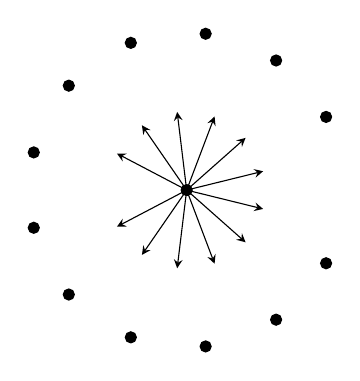
\begin{tikzpicture}
					\def\R{2};
				
					\foreach \i in {1,...,12}
					{
						\filldraw ({\i*360/13}:\R) circle [radius = 2pt];
						\draw [-stealth] (0,0) -- ($ (0,0) ! -1cm ! ({\i*360/13}:\R)$);
					}
				
					\filldraw (0,0) circle [radius = 2pt];
				\end{tikzpicture}
			\end{figure}
			If one of the 13 charges is removed, the net force on $Q$ will be equal to the force due to the removed $q$, which was previously acting on it.\\
			Therefore,
			\begin{align*}
				F &= \dfrac{k Q q}{r^2}
			\end{align*}
			in the direction of the removed charge.
	\end{tasks}
\end{solution}

\begin{question}
	\begin{tasks}
		\task
			\label{1}
			Find the electric field (magnitude and direction) a distance $z$ above the midpoint between two equal charges, $q$, a distance $d$ apart. Check that your result is consistent with what you'd expect when $z >> d$.
		\task
			Repeat part \ref{1}, only this time make the right-hand charge $-q$ instead of $+q$.
	\end{tasks}
\end{question}

\begin{solution}
	\begin{tasks}
		\task
			\begin{figure}[H]
				\begin{tikzpicture}
					\def\z{3};
					\def\d{4};
					
					\coordinate (q1) at ({-\d/2},0);
					\coordinate (q2) at ({\d/2},0);
					\coordinate (P) at (0,\z);
					
					\begin{scope}
						\filldraw (q1) circle (2pt) node [below] {$q$};
						\filldraw (q2) circle (2pt) node [below] {$q$};
						
						\filldraw (P) circle (1pt);
					\end{scope}
					
					\begin{scope}
						\draw ($ (q1) + (-1,0) $) -- ($ (q2) + (1,0) $);
						\draw ($ (P) + (0,1) $) -- (0,-1);
					\end{scope}
					
					\begin{scope}[-stealth]
						\draw (P) -- ($ (P) ! -1cm ! (q1) $) node [above right] {$E$};
						\draw (P) -- ($ (P) ! -1cm ! (q2) $) node [above left] {$E$};
					\end{scope}
				\end{tikzpicture}
			\end{figure}
			Let the angle between $E$ and the vertical direction be $\theta$.\\
			By symmetry, the horizontal components of the fields will cancel out and the vertical components will add up.\\
			Therefore,
			\begin{align*}
				\overrightarrow{E_{\textnormal{net}}} &= 2 E \cos \theta \hat{z}\\
				&= \dfrac{2 k q}{\dfrac{d^2}{4} + z^2} \cdot \dfrac{z}{\sqrt{\dfrac{d^2}{4} + z^2}}\\
				&= \dfrac{2 k q z}{\left( \dfrac{d^2}{4} + z^2 \right)^{\sfrac{3}{2}}}
			\end{align*}
			If $z >> d$,
			\begin{align*}
				\overrightarrow{E_{\textnormal{net}}} &= \dfrac{2 k q z}{z^3}\\
				&= \dfrac{2 k q}{z^2}
			\end{align*}
			This is equivalent to the field at $z$ due to a point charge $2q$. Thus, this result is consistent with Coulomb's Law for point charges.
		\task
			\begin{figure}[H]
				\begin{tikzpicture}
					\def\z{3};
					\def\d{4};
					
					\coordinate (q1) at ({-\d/2},0);
					\coordinate (q2) at ({\d/2},0);
					\coordinate (P) at (0,\z);
					
					\begin{scope}
						\filldraw (q1) circle (2pt) node [below] {$q$};
						\filldraw (q2) circle (2pt) node [below] {$-q$};
						
						\filldraw (P) circle (1pt);
					\end{scope}
					
					\begin{scope}
						\draw ($ (q1) + (-1,0) $) -- ($ (q2) + (1,0) $);
						\draw ($ (P) + (0,1) $) -- (0,-1);
					\end{scope}
					
					\begin{scope}[-stealth]
						\draw (P) -- ($ (P) ! -1cm ! (q1) $) node [above right] {$E$};
						\draw (P) -- ($ (P) ! 1cm ! (q2) $) node [below right] {$E$};
					\end{scope}
				\end{tikzpicture}
			\end{figure}
			Let the angle between $E$ and the vertical direction be $\theta$.\\
			By symmetry, the vertical components of the fields will cancel out and the horizontal components will add up.\\
			Therefore,
			\begin{align*}
				\overrightarrow{E_{\textnormal{net}}} &= 2 E \sin \theta \hat{z}\\
				&= \dfrac{2 k q}{\dfrac{d^2}{4} + z^2} \cdot \dfrac{\dfrac{d}{2}}{\sqrt{\dfrac{d^2}{4} + z^2}}\\
				&= \dfrac{2 k q d}{\left( \dfrac{d^2}{4} + z^2 \right)^{\sfrac{3}{2}}}
			\end{align*}
			If $z >> d$,
			\begin{align*}
				\overrightarrow{E_{\textnormal{net}}} &= 0
			\end{align*}
			This is equivalent to a field at $z$ due to a neutral point charge. Thus, this result is consistent with Coulomb's Law for point charges.
	\end{tasks}
\end{solution}

\begin{question}
		Find the electric field a distance $z$ above the centre of a square loop of side $a$ carrying uniform line charge $\lambda$.
\end{question}

\begin{solution}
	Let $F$ be the field at $P$ due to one side.
	Let the angle between $\overrightarrow{F}$ and $\hat{z}$ be $\theta$.
	Therefore, due to symmetry, the net field at $P$ due to all four sides will be $4 F \cos \theta$.
	\begin{figure}[H]
		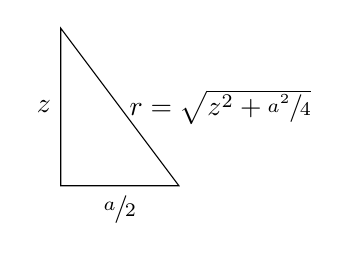
\begin{tikzpicture}
			\def\z{2};
			\def\a{3};
			
			\draw (0,0) -- node [midway, left] {$z$} (0,\z) -- node [midway, right] {$r = \sqrt{z^2 + \sfrac{a^2}{4}}$} ({\a/2},0) -- node [midway, below] {$\sfrac{a}{2}$} cycle;
		\end{tikzpicture}
	\end{figure}
	Therefore,
	\begin{align*}
		F &= k \dfrac{\lambda a}{r \left( \sfrac{a^2}{4} + r^2 \right)^{\sfrac{1}{2}}}\\
		\therefore F_{\textnormal{net}} &= 4 k \dfrac{\lambda a}{r \left( \sfrac{a^2}{4} + r^2 \right)^{\sfrac{1}{2}}} \cdot \dfrac{\sfrac{a}{2}}{r}\\
		&= 2 k \dfrac{\lambda a^2}{r^2 \left( \sfrac{a^2}{4} + r^2 \right)^{\sfrac{1}{2}}}
	\end{align*}
\end{solution}

\begin{question}
	Find the electric field a distance $z$ above the centre of a flat circular disk of radius $R$, which carries a uniform surface charge $\sigma$. What does your formula give in the limit $R \to \infty$? Also check the case $z >> R$.
\end{question}

\begin{solution}
	Consider an elemental ring of radius $r$ and thickness $\dif r$.
	Therefore,
	\begin{align*}
		\dif q &= \sigma \cdot 2 \pi r \dif r\\
		\therefore \dif E &= \dfrac{k z \dif q}{\left( z^2 + r^2 \right)^{\sfrac{3}{2}}}\\
		&= \dfrac{2 \sigma \pi z r \dif r}{4 \pi \varepsilon_0 \left( z^2 + r^2 \right)^{\sfrac{3}{2}}}\\
		&= \dfrac{z \sigma r \dif r}{2 \varepsilon_0 \left( z^2 + r^2 \right)^{\sfrac{3}{2}}}\\
		\therefore E &= \dfrac{z \sigma}{2 \varepsilon_0} \int\limits_{0}^{R} \dfrac{r \dif r}{\left( z^2 + r^2 \right)^{\sfrac{3}{2}}}\\
		&= \dfrac{z \sigma}{2 \varepsilon_0} \left[ \dfrac{-1}{\sqrt{z^2 + r^2}} \right]_{0}^{R}\\
		&= \dfrac{z \sigma}{2 \varepsilon_0} \left( \dfrac{-1}{\sqrt{z^2 + R^2}} + \dfrac{1}{z} \right)\\
		&= \dfrac{z \sigma}{2 \varepsilon_0} \left( \dfrac{1}{z} - \dfrac{1}{\sqrt{z^2 + R^2}} \right)
	\end{align*}
	~\\
	If $R \to \infty$,
	\begin{align*}
		E &= \dfrac{z \sigma}{2 \varepsilon_0} \left( \dfrac{1}{z} \right)\\
		&= \dfrac{\sigma}{2 \varepsilon_0}
	\end{align*}
	This is consistent with the value of electric field due to an infinite plane of charge.
\end{solution}

\begin{question}
	Find the electric field a distance z from the centre of a spherical surface of radius $R$, which carries a uniform charge density $\sigma$.
\end{question}

\begin{solution}
	\begin{align*}
		\dif q &= \sigma R^2 \sin \theta \dif \theta \dif \varphi\\
		\therefore \dif E &= k \dfrac{\dif q}{R^2 + z^2 - 2 R z \cos \theta}
	\end{align*}
	Due to symmetry, only the components of all $\dif E$ in the $z$ direction will add up, and all other components will cancel out.\\
	Let the angle between $\overrightarrow{\dif E}$ and the $z$-axis be $\alpha$.\\
	Therefore,
	\begin{align*}
		\cos \alpha &= \dfrac{z - R \cos \theta}{\sqrt{R^2 + z^2 - 2 R z \cos \theta}}
	\end{align*}
	Therefore,
	\begin{align*}
		E &= \int \dif E \cos \alpha\\
		&= \int\limits_{0}^{2 \pi} \int\limits_{0}^{\pi} \dfrac{k \sigma R^2 \sin \theta (z - R \cos \theta)}{\left( R^2 + z^2 - 2 R z \cos \theta \right)^{\sfrac{3}{2}}} \dif \theta \dif \varphi
	\end{align*}
	Integrating,\\
	If $z = R$,
	\begin{align*}
		E &= \dfrac{k q}{R^2}
	\end{align*}
	Else,
	\begin{align*}
		E &= \dfrac{k q}{4 R z^2} \left( (z + R) - |z - R| - (z^2 + R^2) \left( \dfrac{1}{z + R} - \dfrac{1}{|z - R|} \right) \right)
	\end{align*}
	Therefore,
	\begin{align*}
		E &= 
			\begin{cases}
				0 &;\quad z < R\\
				\dfrac{k q}{z^2} &;\quad z \geq R\\
			\end{cases}
	\end{align*}
\end{solution}

\begin{question}
	Find the field inside and outside a sphere of radius $R$, which carries a uniform volume charge density $\rho$.
\end{question}

\begin{solution}
	 From the previous result, if $z < R$, only the part of the sphere on the inside, i.e. the smaller sphere of radius $z$ will have an effect on the field at the point.
	 The part of the sphere outside will have no field at the point.\\
	 \begin{align*}
	 	 E &= \int \dfrac{k \dif q}{z^2}\\
	 	 &= \int\limits_{0}^{z} \dfrac{k \rho \cdot 4 \pi}{R^2} \cdot r^2 \dif r\\
	 	 &= \dfrac{k q z}{R^3}
	 \end{align*}
	 If $z \geq R$, the whole sphere will affect the field.\\
	 Therefore, by the previous result,
	\begin{align*}
		E &= \dfrac{k q}{R^2}
	\end{align*}
	Therefore,
	\begin{align*}
		E &= 
			\begin{cases}
				\dfrac{k q}{z^2} &;\quad z \geq R\\
				\dfrac{k q z}{R^2} &;\quad z \leq R\\
			\end{cases}
	\end{align*}
	\begin{figure}[H]
		\begin{tikzpicture}
			\def\R{2};
			\def\surfaceE{2};
			
			\begin{scope}[stealth-stealth]
				\draw (-1,0) -- ({3*\R + 1},0) node [below] {distance from centre};
				\draw (0,-1) -- (0,{\surfaceE + 1}) node [above] {$|E|$};
			\end{scope}
			
			\begin{scope}[dashed]
				\draw (\R,\surfaceE) to (\R,0) node [below] {$R$};
				\draw (\R,\surfaceE) to (0,\surfaceE) node [left] {$\dfrac{k q}{R^2}$};
			\end{scope}
			
			\begin{scope}
				\draw (0,0) -- (\R,\surfaceE);
				\draw (\R,\surfaceE) to [out = -80, in = 180] ({3*\R}, 0.1);
			\end{scope}
		\end{tikzpicture}
	\end{figure}
\end{solution}

\end{document}